\documentclass[11pt,a4paper]{article}

% ============================================================================
% PACKAGES
% ============================================================================
\usepackage[utf8]{inputenc}
\usepackage[T1]{fontenc}
\usepackage{lmodern}
\usepackage[margin=1in]{geometry}
\usepackage{graphicx}
\usepackage{xcolor}
\usepackage{hyperref}
\usepackage{listings}
\usepackage{booktabs}
\usepackage{longtable}
\usepackage{array}
\usepackage{tikz}
\usepackage{float}
\usepackage{enumitem}
\usepackage{amsmath}
\usepackage{amssymb}
\usepackage{fancyhdr}
\usepackage{tocloft}
\usepackage{caption}
\usepackage{subcaption}

% TikZ Libraries
\usetikzlibrary{shapes.geometric, arrows.meta, positioning, fit, backgrounds, calc, decorations.pathreplacing}

% ============================================================================
% STYLING
% ============================================================================
\definecolor{primaryblue}{RGB}{41, 128, 185}
\definecolor{secondarygreen}{RGB}{39, 174, 96}
\definecolor{accentorange}{RGB}{230, 126, 34}
\definecolor{darkgray}{RGB}{52, 73, 94}
\definecolor{lightgray}{RGB}{236, 240, 241}
\definecolor{codebg}{RGB}{248, 249, 250}
\definecolor{codeframe}{RGB}{200, 200, 200}

\hypersetup{
    colorlinks=true,
    linkcolor=primaryblue,
    urlcolor=primaryblue,
    citecolor=primaryblue,
    pdftitle={XAI-Lab Technical Documentation},
    pdfauthor={XAI-Lab Team}
}

% Code listing style
\lstdefinestyle{pythonstyle}{
    backgroundcolor=\color{codebg},
    basicstyle=\ttfamily\small,
    breakatwhitespace=false,
    breaklines=true,
    captionpos=b,
    commentstyle=\color{secondarygreen},
    frame=single,
    framerule=0.5pt,
    rulecolor=\color{codeframe},
    keywordstyle=\color{primaryblue}\bfseries,
    language=Python,
    numbers=left,
    numbersep=8pt,
    numberstyle=\tiny\color{gray},
    showspaces=false,
    showstringspaces=false,
    stringstyle=\color{accentorange},
    tabsize=4,
    xleftmargin=15pt
}

\lstdefinestyle{yamlstyle}{
    backgroundcolor=\color{codebg},
    basicstyle=\ttfamily\small,
    breaklines=true,
    frame=single,
    framerule=0.5pt,
    rulecolor=\color{codeframe},
    keywordstyle=\color{primaryblue},
    numbers=left,
    numbersep=8pt,
    numberstyle=\tiny\color{gray},
    xleftmargin=15pt
}

\lstset{style=pythonstyle}

% Header/Footer
\pagestyle{fancy}
\fancyhf{}
\fancyhead[L]{\textcolor{darkgray}{\small XAI-Lab Documentation}}
\fancyhead[R]{\textcolor{darkgray}{\small \leftmark}}
\fancyfoot[C]{\textcolor{darkgray}{\thepage}}
\renewcommand{\headrulewidth}{0.4pt}
\renewcommand{\footrulewidth}{0.4pt}

% ============================================================================
% DOCUMENT
% ============================================================================
\begin{document}

% ----------------------------------------------------------------------------
% TITLE PAGE
% ----------------------------------------------------------------------------
\begin{titlepage}
    \centering
    \vspace*{2cm}

    {\Huge\bfseries\textcolor{primaryblue}{XAI-Lab}}\\[0.5cm]
    {\LARGE\textcolor{darkgray}{Credit Risk Prediction Platform}}\\[0.3cm]
    {\Large\textcolor{darkgray}{with Explainable AI \& Fairness Auditing}}\\[2cm]

    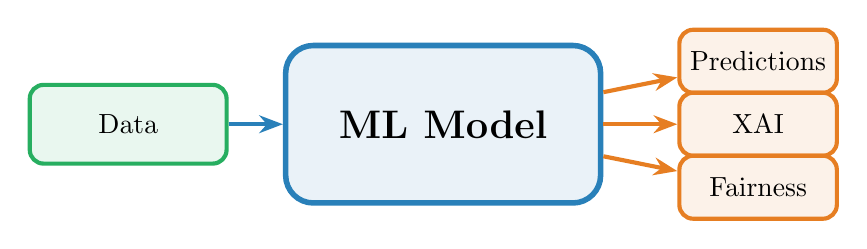
\begin{tikzpicture}[scale=0.8]
        % Central ML icon
        \node[draw=primaryblue, fill=primaryblue!10, rounded corners=10pt, minimum width=4cm, minimum height=2cm, line width=2pt] (ml) at (0,0) {\Large\textbf{ML Model}};

        % Input
        \node[draw=secondarygreen, fill=secondarygreen!10, rounded corners=5pt, minimum width=2.5cm, minimum height=1cm, line width=1.5pt] (data) at (-5,0) {Data};

        % Outputs
        \node[draw=accentorange, fill=accentorange!10, rounded corners=5pt, minimum width=2cm, minimum height=0.8cm, line width=1.5pt] (pred) at (5,1) {Predictions};
        \node[draw=accentorange, fill=accentorange!10, rounded corners=5pt, minimum width=2cm, minimum height=0.8cm, line width=1.5pt] (xai) at (5,0) {XAI};
        \node[draw=accentorange, fill=accentorange!10, rounded corners=5pt, minimum width=2cm, minimum height=0.8cm, line width=1.5pt] (fair) at (5,-1) {Fairness};

        % Arrows
        \draw[-{Stealth[length=3mm]}, line width=1.5pt, primaryblue] (data) -- (ml);
        \draw[-{Stealth[length=3mm]}, line width=1.5pt, accentorange] (ml) -- (pred);
        \draw[-{Stealth[length=3mm]}, line width=1.5pt, accentorange] (ml) -- (xai);
        \draw[-{Stealth[length=3mm]}, line width=1.5pt, accentorange] (ml) -- (fair);
    \end{tikzpicture}

    \vfill

    {\Large\textcolor{darkgray}{Technical Documentation}}\\[0.5cm]
    {\large Version 1.0}\\[1cm]

    \rule{0.6\textwidth}{0.4pt}\\[0.5cm]
    {\large\today}

\end{titlepage}

% ----------------------------------------------------------------------------
% TABLE OF CONTENTS
% ----------------------------------------------------------------------------
\tableofcontents
\newpage

% ============================================================================
% SECTION 1: EXECUTIVE SUMMARY
% ============================================================================
\section{Executive Summary}

XAI-Lab is a production-ready \textbf{Credit Risk Prediction Platform} that combines machine learning with explainable AI (XAI) and algorithmic fairness auditing. The platform addresses the critical need for transparent, interpretable, and fair automated credit decisions in financial services.

\subsection{Key Capabilities}

\begin{itemize}[leftmargin=*]
    \item \textbf{Credit Risk Classification}: Binary classification (Good/Bad risk) using XGBoost
    \item \textbf{Explainable AI}: SHAP and LIME explanations for model interpretability
    \item \textbf{Fairness Auditing}: Gender-based fairness metrics using Fairlearn
    \item \textbf{Experiment Tracking}: MLflow integration for reproducibility
    \item \textbf{Production Deployment}: Docker Compose and Kubernetes support
    \item \textbf{Model Hot-Reload}: Zero-downtime model updates in production
\end{itemize}

\subsection{Technology Stack}

\begin{table}[H]
\centering
\begin{tabular}{@{}ll@{}}
\toprule
\textbf{Category} & \textbf{Technologies} \\
\midrule
Machine Learning & XGBoost, scikit-learn \\
Explainability & SHAP, LIME \\
Fairness & Fairlearn \\
Experiment Tracking & MLflow \\
API Framework & FastAPI, Flask \\
Containerization & Docker, Docker Compose \\
Orchestration & Kubernetes (with HPA) \\
\bottomrule
\end{tabular}
\caption{Technology stack overview}
\end{table}

% ============================================================================
% SECTION 2: PROJECT OBJECTIVES
% ============================================================================
\section{Project Objectives}

\subsection{Primary Goals}

The XAI-Lab platform is designed to demonstrate and implement:

\begin{enumerate}[leftmargin=*]
    \item \textbf{Responsible AI Development}: Building ML systems that are transparent, fair, and accountable
    \item \textbf{Production MLOps}: End-to-end pipeline from training to deployment with proper versioning
    \item \textbf{Regulatory Compliance}: Meeting requirements for explainability in automated decision-making (e.g., GDPR Article 22, Fair Lending laws)
    \item \textbf{Scalable Architecture}: Microservices design supporting horizontal scaling
\end{enumerate}

\subsection{Business Context}

Credit risk assessment is a critical financial application where:
\begin{itemize}
    \item Decisions directly impact individuals' access to financial services
    \item Regulatory bodies require explanation of automated decisions
    \item Historical biases in data can perpetuate discrimination
    \item Model performance must be continuously monitored
\end{itemize}

% ============================================================================
% SECTION 3: SYSTEM ARCHITECTURE
% ============================================================================
\section{System Architecture}

\subsection{High-Level Architecture}

The system follows a microservices architecture with clear separation of concerns between training, evaluation, and inference components.

\begin{figure}[H]
\centering
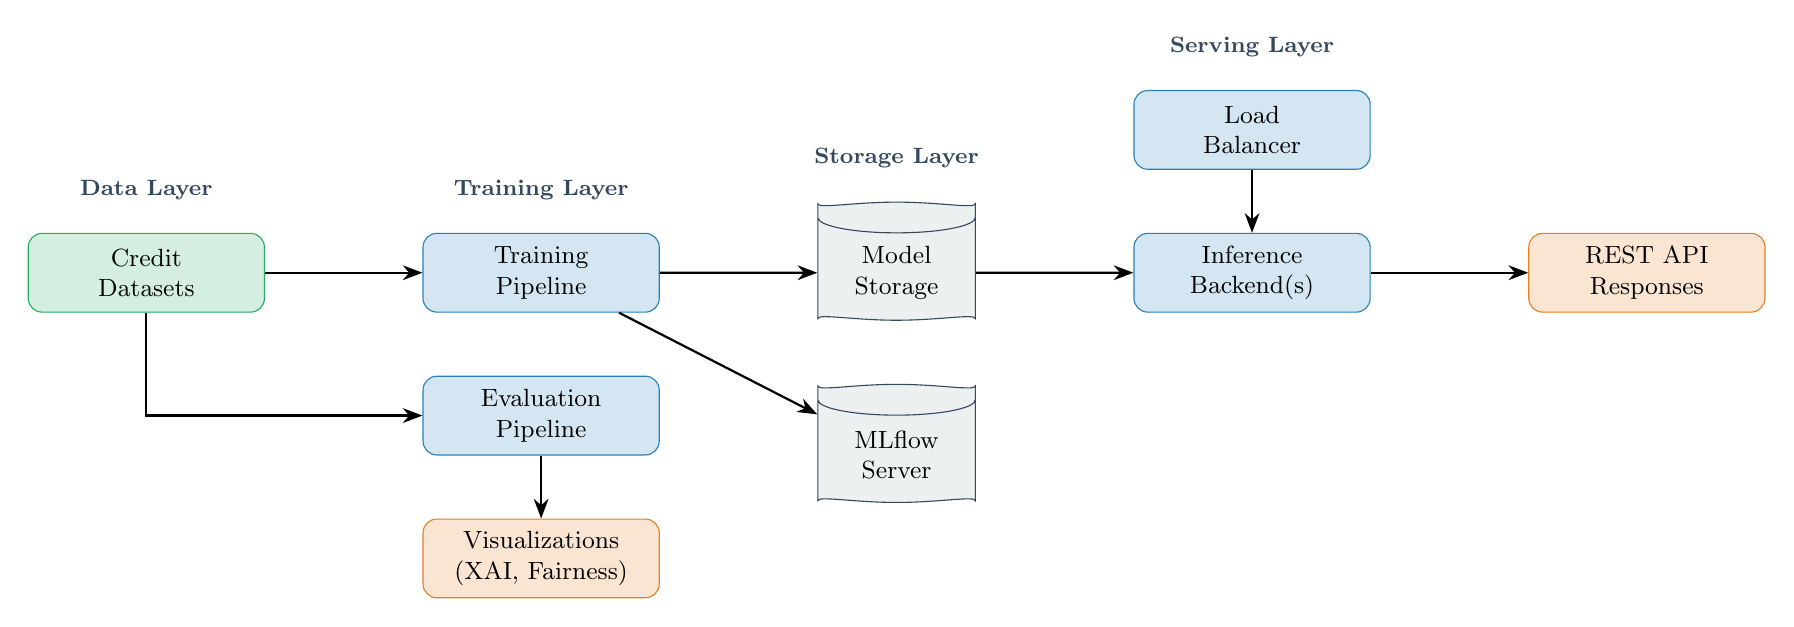
\begin{tikzpicture}[
    node distance=1.5cm,
    component/.style={draw, rounded corners=5pt, minimum width=3cm, minimum height=1cm, align=center, font=\small},
    data/.style={component, fill=secondarygreen!20, draw=secondarygreen},
    process/.style={component, fill=primaryblue!20, draw=primaryblue},
    output/.style={component, fill=accentorange!20, draw=accentorange},
    storage/.style={component, fill=lightgray, draw=darkgray, cylinder, shape border rotate=90, aspect=0.3},
    arrow/.style={-{Stealth[length=2.5mm]}, thick}
]

% Data Layer
\node[data] (dataset) {Credit\\Datasets};

% Training Pipeline
\node[process, right=2cm of dataset] (train) {Training\\Pipeline};
\node[process, below=0.8cm of train] (eval) {Evaluation\\Pipeline};

% Storage
\node[storage, right=2cm of train, minimum width=2cm, minimum height=1.5cm] (model) {Model\\Storage};
\node[storage, below=0.8cm of model, minimum width=2cm, minimum height=1.5cm] (mlflow) {MLflow\\Server};

% Inference
\node[process, right=2cm of model] (backend) {Inference\\Backend(s)};
\node[process, above=0.8cm of backend] (lb) {Load\\Balancer};

% Outputs
\node[output, right=2cm of backend] (api) {REST API\\Responses};
\node[output, below=0.8cm of eval] (viz) {Visualizations\\(XAI, Fairness)};

% Arrows
\draw[arrow] (dataset) -- (train);
\draw[arrow] (dataset) |- (eval);
\draw[arrow] (train) -- (model);
\draw[arrow] (train) -- (mlflow);
\draw[arrow] (eval) -- (viz);
\draw[arrow] (model) -- (backend);
\draw[arrow] (lb) -- (backend);
\draw[arrow] (backend) -- (api);

% Labels
\node[above=0.3cm of dataset, font=\footnotesize\bfseries, text=darkgray] {Data Layer};
\node[above=0.3cm of train, font=\footnotesize\bfseries, text=darkgray] {Training Layer};
\node[above=0.3cm of model, font=\footnotesize\bfseries, text=darkgray] {Storage Layer};
\node[above=0.3cm of lb, font=\footnotesize\bfseries, text=darkgray] {Serving Layer};

\end{tikzpicture}
\caption{High-level system architecture}
\label{fig:high-level-arch}
\end{figure}

\subsection{Component Overview}

\begin{table}[H]
\centering
\small
\begin{tabular}{@{}p{3cm}p{3cm}p{7cm}@{}}
\toprule
\textbf{Component} & \textbf{File(s)} & \textbf{Responsibility} \\
\midrule
Configuration & \texttt{config.py} & Central configuration for paths, features, and data schema \\
Training & \texttt{train.py} & XGBoost model training with sklearn Pipeline \\
Evaluation & \texttt{evaluate.py} & Performance metrics, XAI (SHAP/LIME), fairness analysis \\
MLflow Logger & \texttt{mlflow\_logger.py} & Experiment tracking and artifact logging \\
Inference API & \texttt{inference.py} & Simple FastAPI endpoint for predictions \\
K8s Backend & \texttt{backend.py} & Production backend with model hot-reload \\
Load Balancer & \texttt{load\_balancer.py} & Round-robin request distribution \\
K8s Trainer & \texttt{model\_trainer.py} & CronJob-compatible training script \\
\bottomrule
\end{tabular}
\caption{Component responsibilities}
\end{table}

\subsection{Data Flow Diagram}

\begin{figure}[H]
\centering
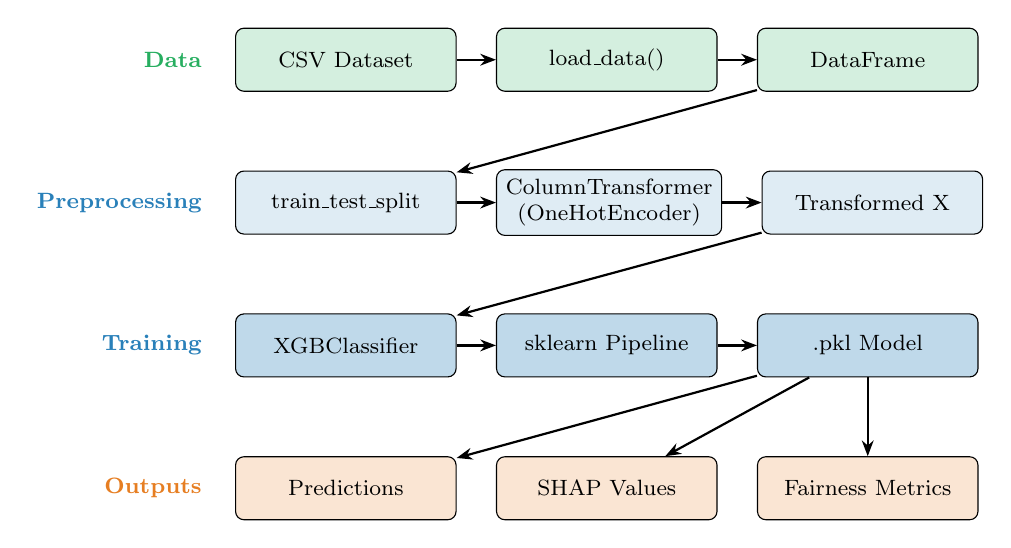
\begin{tikzpicture}[
    node distance=0.8cm,
    box/.style={draw, rounded corners=3pt, minimum width=2.8cm, minimum height=0.8cm, align=center, font=\footnotesize},
    arrow/.style={-{Stealth[length=2mm]}, thick},
    label/.style={font=\tiny, text=gray}
]

% Row 1: Data
\node[box, fill=secondarygreen!20] (csv) {CSV Dataset};
\node[box, fill=secondarygreen!20, right=0.5cm of csv] (load) {load\_data()};
\node[box, fill=secondarygreen!20, right=0.5cm of load] (df) {DataFrame};

% Row 2: Preprocessing
\node[box, fill=primaryblue!15, below=1cm of csv] (split) {train\_test\_split};
\node[box, fill=primaryblue!15, right=0.5cm of split] (preproc) {ColumnTransformer\\(OneHotEncoder)};
\node[box, fill=primaryblue!15, right=0.5cm of preproc] (xtrans) {Transformed X};

% Row 3: Model
\node[box, fill=primaryblue!30, below=1cm of split] (xgb) {XGBClassifier};
\node[box, fill=primaryblue!30, right=0.5cm of xgb] (pipeline) {sklearn Pipeline};
\node[box, fill=primaryblue!30, right=0.5cm of pipeline] (pkl) {.pkl Model};

% Row 4: Outputs
\node[box, fill=accentorange!20, below=1cm of xgb] (pred) {Predictions};
\node[box, fill=accentorange!20, right=0.5cm of pred] (shap) {SHAP Values};
\node[box, fill=accentorange!20, right=0.5cm of shap] (fair) {Fairness Metrics};

% Arrows
\draw[arrow] (csv) -- (load);
\draw[arrow] (load) -- (df);
\draw[arrow] (df) -- (split);
\draw[arrow] (split) -- (preproc);
\draw[arrow] (preproc) -- (xtrans);
\draw[arrow] (xtrans) -- (xgb);
\draw[arrow] (xgb) -- (pipeline);
\draw[arrow] (pipeline) -- (pkl);
\draw[arrow] (pkl) -- (pred);
\draw[arrow] (pkl) -- (shap);
\draw[arrow] (pkl) -- (fair);

% Stage labels
\node[left=0.3cm of csv, font=\footnotesize\bfseries, text=secondarygreen] {Data};
\node[left=0.3cm of split, font=\footnotesize\bfseries, text=primaryblue] {Preprocessing};
\node[left=0.3cm of xgb, font=\footnotesize\bfseries, text=primaryblue] {Training};
\node[left=0.3cm of pred, font=\footnotesize\bfseries, text=accentorange] {Outputs};

\end{tikzpicture}
\caption{Data flow through the training pipeline}
\label{fig:data-flow}
\end{figure}

% ============================================================================
% SECTION 4: DATA SCHEMA
% ============================================================================
\section{Data Schema and Feature Engineering}

\subsection{Dataset Structure}

The platform uses credit risk datasets with the following schema:

\begin{table}[H]
\centering
\begin{tabular}{@{}llll@{}}
\toprule
\textbf{Feature} & \textbf{Type} & \textbf{Category} & \textbf{Description} \\
\midrule
Age & Integer & Numerical & Applicant's age \\
Sex & String & Categorical & Gender (male/female) — \textit{protected attribute} \\
Job & Integer & Numerical & Job category (0-3) \\
Housing & String & Categorical & Ownership status (own/rent/free) \\
Saving accounts & String & Categorical & Savings level (little/moderate/quite rich/rich) \\
Checking account & Float & Numerical & Checking account balance indicator \\
Credit amount & Float & Numerical & Requested credit amount \\
Duration & Integer & Numerical & Loan duration in months \\
Purpose & String & Categorical & Loan purpose (car/education/etc.) \\
\midrule
Risk & String & \textbf{Target} & Credit risk label (Good/Bad) \\
\bottomrule
\end{tabular}
\caption{Dataset schema}
\end{table}

\subsection{Feature Configuration}

The \texttt{config.py} file defines feature sets:

\begin{lstlisting}[style=pythonstyle]
# Control gender inclusion in model
WITH_GENDER = True  # Set to False to exclude gender

# Feature definitions
CATEGORICAL_COLS = ["Sex", "Housing", "Saving accounts", "Purpose"]
NUMERICAL_COLS = ["Age", "Job", "Checking account",
                  "Credit amount", "Duration"]

# Target encoding
def encode_target(y: pd.Series) -> pd.Series:
    return y.map({"Good": 1, "Bad": 0})
\end{lstlisting}

\subsection{Preprocessing Pipeline}

The preprocessing uses scikit-learn's \texttt{ColumnTransformer}:

\begin{figure}[H]
\centering
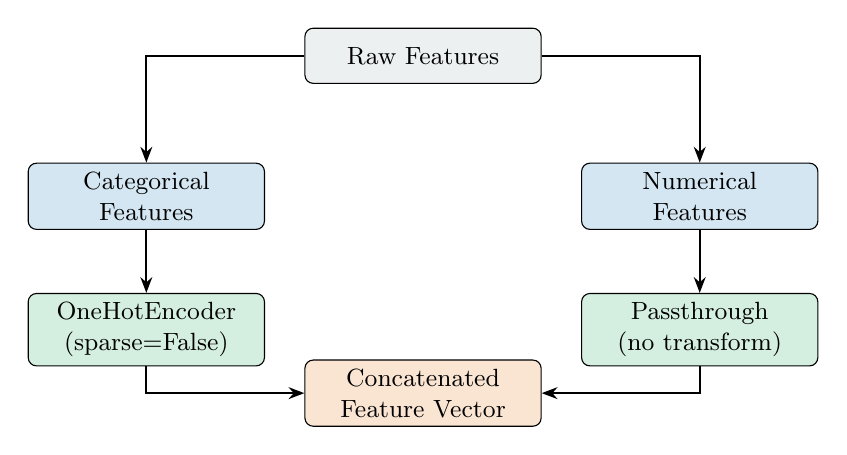
\begin{tikzpicture}[
    node distance=0.5cm,
    box/.style={draw, rounded corners=3pt, minimum width=3cm, minimum height=0.7cm, align=center, font=\small},
    arrow/.style={-{Stealth[length=2mm]}, thick}
]

\node[box, fill=lightgray] (input) {Raw Features};

\node[box, fill=primaryblue!20, below left=1cm and 0.5cm of input] (cat) {Categorical\\Features};
\node[box, fill=primaryblue!20, below right=1cm and 0.5cm of input] (num) {Numerical\\Features};

\node[box, fill=secondarygreen!20, below=0.8cm of cat] (ohe) {OneHotEncoder\\(sparse=False)};
\node[box, fill=secondarygreen!20, below=0.8cm of num] (pass) {Passthrough\\(no transform)};

\node[box, fill=accentorange!20, below=1.5cm of input, yshift=-2cm] (concat) {Concatenated\\Feature Vector};

\draw[arrow] (input) -| (cat);
\draw[arrow] (input) -| (num);
\draw[arrow] (cat) -- (ohe);
\draw[arrow] (num) -- (pass);
\draw[arrow] (ohe) |- (concat);
\draw[arrow] (pass) |- (concat);

\end{tikzpicture}
\caption{Preprocessing pipeline structure}
\end{figure}

% ============================================================================
% SECTION 5: MACHINE LEARNING MODEL
% ============================================================================
\section{Machine Learning Model}

\subsection{Model Architecture}

The platform uses \textbf{XGBoost (eXtreme Gradient Boosting)} for binary classification:

\begin{lstlisting}[style=pythonstyle]
model = XGBClassifier(
    n_estimators=200,      # Number of boosting rounds
    max_depth=4,           # Maximum tree depth
    learning_rate=0.1,     # Step size shrinkage
    subsample=0.9,         # Row sampling ratio
    colsample_bytree=0.9,  # Column sampling ratio
    random_state=42,       # Reproducibility seed
    n_jobs=-1,             # Use all CPU cores
    objective="binary:logistic",
    eval_metric="logloss",
)
\end{lstlisting}

\subsection{Why XGBoost?}

\begin{itemize}
    \item \textbf{Performance}: State-of-the-art results on tabular data
    \item \textbf{Interpretability}: Native feature importance; compatible with SHAP TreeExplainer
    \item \textbf{Robustness}: Handles missing values and mixed feature types
    \item \textbf{Efficiency}: Fast training and inference
\end{itemize}

\subsection{Training Pipeline}

\begin{lstlisting}[style=pythonstyle]
# Complete pipeline wraps preprocessing + model
pipeline = Pipeline([
    ("preprocessor", preprocessor),  # ColumnTransformer
    ("model", model),                # XGBClassifier
])

# Train with stratified split
X_train, X_test, y_train, y_test = train_test_split(
    X, y, test_size=0.2, stratify=y, random_state=42
)

pipeline.fit(X_train, y_train)
joblib.dump(pipeline, "model/xgb_credit_model.pkl")
\end{lstlisting}

\subsection{Model Performance Metrics}

The evaluation pipeline computes:

\begin{table}[H]
\centering
\begin{tabular}{@{}ll@{}}
\toprule
\textbf{Metric} & \textbf{Description} \\
\midrule
Accuracy & Overall correct predictions \\
Precision & True positives / Predicted positives \\
Recall & True positives / Actual positives \\
F1 Score (Macro) & Harmonic mean of precision and recall \\
ROC AUC & Area under ROC curve \\
\bottomrule
\end{tabular}
\caption{Performance metrics tracked}
\end{table}

% ============================================================================
% SECTION 6: EXPLAINABLE AI (XAI)
% ============================================================================
\section{Explainable AI (XAI)}

\subsection{Why Explainability Matters}

In credit risk assessment, explainability is essential for:
\begin{itemize}
    \item \textbf{Regulatory Compliance}: GDPR's ``right to explanation'' (Article 22)
    \item \textbf{Trust Building}: Stakeholders need to understand model decisions
    \item \textbf{Model Debugging}: Identifying unexpected feature dependencies
    \item \textbf{Bias Detection}: Understanding how protected attributes influence predictions
\end{itemize}

\subsection{SHAP (SHapley Additive exPlanations)}

SHAP provides \textbf{global} and \textbf{local} feature importance based on game theory.

\begin{figure}[H]
\centering
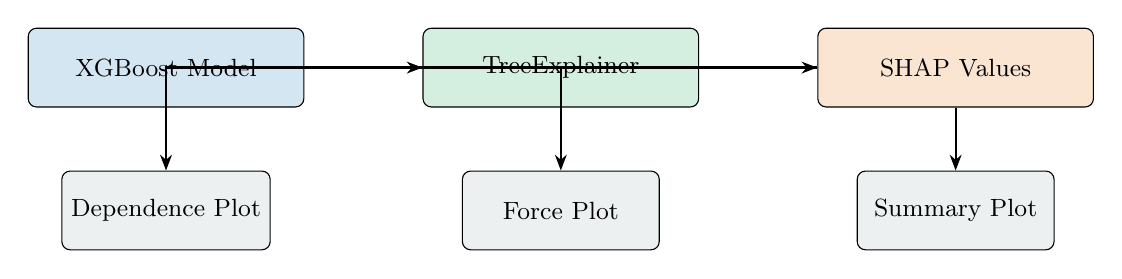
\begin{tikzpicture}[
    node distance=0.8cm,
    box/.style={draw, rounded corners=3pt, minimum width=3.5cm, minimum height=1cm, align=center, font=\small},
    arrow/.style={-{Stealth[length=2mm]}, thick}
]

\node[box, fill=primaryblue!20] (model) {XGBoost Model};
\node[box, fill=secondarygreen!20, right=1.5cm of model] (explainer) {TreeExplainer};
\node[box, fill=accentorange!20, right=1.5cm of explainer] (values) {SHAP Values};

\node[box, fill=lightgray, below=0.8cm of values, minimum width=2.5cm] (summary) {Summary Plot};
\node[box, fill=lightgray, below=0.8cm of explainer, minimum width=2.5cm] (force) {Force Plot};
\node[box, fill=lightgray, below=0.8cm of model, minimum width=2.5cm] (depend) {Dependence Plot};

\draw[arrow] (model) -- (explainer);
\draw[arrow] (explainer) -- (values);
\draw[arrow] (values) -- (summary);
\draw[arrow] (values) -| (force);
\draw[arrow] (values) -| (depend);

\end{tikzpicture}
\caption{SHAP explanation pipeline}
\end{figure}

\textbf{Implementation:}
\begin{lstlisting}[style=pythonstyle]
# Create TreeExplainer for XGBoost
explainer = shap.TreeExplainer(model.get_booster())

# Compute SHAP values for test set
shap_values = explainer.shap_values(X_test_transformed)

# Generate summary plot (global feature importance)
shap.summary_plot(shap_values, X_test_transformed,
                  feature_names=feature_names, show=False)
\end{lstlisting}

\textbf{Key Outputs:}
\begin{itemize}
    \item \textbf{Summary Plot}: Global view of feature importance and impact direction
    \item Shows which features most influence predictions across all samples
    \item Reveals positive/negative correlation with prediction
\end{itemize}

\subsection{LIME (Local Interpretable Model-agnostic Explanations)}

LIME provides \textbf{local} explanations for individual predictions.

\begin{lstlisting}[style=pythonstyle]
# Create LIME explainer
lime_explainer = LimeTabularExplainer(
    training_data=X_train_transformed,
    feature_names=feature_names,
    class_names=["Bad", "Good"],
    mode="classification",
)

# Explain single prediction
explanation = lime_explainer.explain_instance(
    data_row=X_test_transformed[0],
    predict_fn=model.predict_proba,
    num_features=10,
)
\end{lstlisting}

\textbf{SHAP vs LIME Comparison:}

\begin{table}[H]
\centering
\begin{tabular}{@{}p{3cm}p{5cm}p{5cm}@{}}
\toprule
\textbf{Aspect} & \textbf{SHAP} & \textbf{LIME} \\
\midrule
Scope & Global + Local & Local only \\
Approach & Game-theoretic (Shapley values) & Local linear approximation \\
Consistency & Mathematically consistent & Approximate \\
Speed & Fast for tree models & Slower (sampling-based) \\
Best for & Understanding overall model behavior & Explaining individual decisions \\
\bottomrule
\end{tabular}
\caption{SHAP vs LIME comparison}
\end{table}

% ============================================================================
% SECTION 7: FAIRNESS ANALYSIS
% ============================================================================
\section{Fairness Analysis}

\subsection{Why Fairness Matters in Credit}

Algorithmic bias in credit decisions can:
\begin{itemize}
    \item Perpetuate historical discrimination
    \item Violate fair lending regulations (ECOA, Fair Housing Act)
    \item Damage institutional reputation
    \item Exclude deserving applicants from financial services
\end{itemize}

\subsection{Protected Attribute: Gender}

The platform uses \textbf{gender (Sex)} as the protected attribute for fairness analysis. This is controlled by the \texttt{WITH\_GENDER} configuration flag.

\subsection{Fairness Metrics (Fairlearn)}

The platform computes the following fairness metrics:

\begin{figure}[H]
\centering
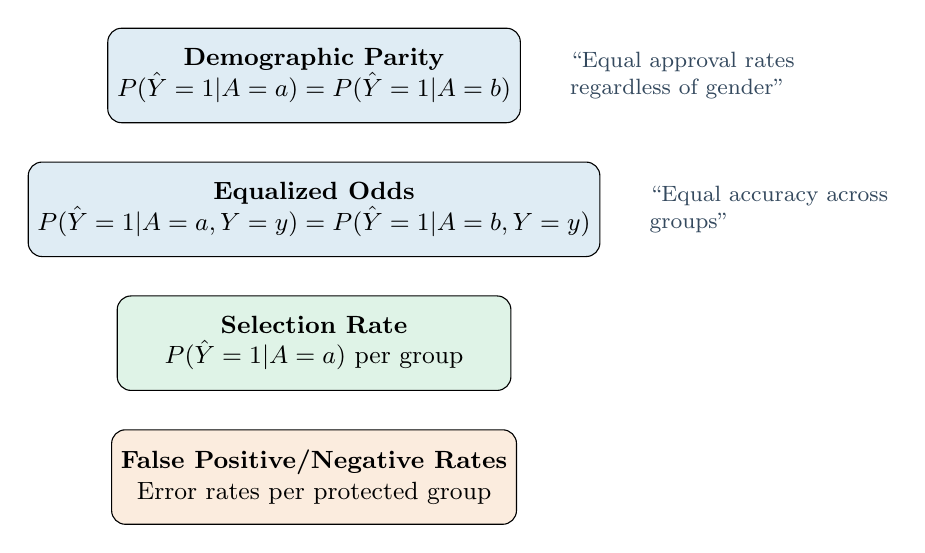
\begin{tikzpicture}[
    metric/.style={draw, rounded corners=5pt, minimum width=5cm, minimum height=1.2cm, align=center, font=\small},
    arrow/.style={-{Stealth[length=2mm]}, thick, dashed}
]

% Group parity metrics
\node[metric, fill=primaryblue!15] (dp) at (0,3) {\textbf{Demographic Parity}\\$P(\hat{Y}=1|A=a) = P(\hat{Y}=1|A=b)$};

\node[metric, fill=primaryblue!15] (eo) at (0,1.3) {\textbf{Equalized Odds}\\$P(\hat{Y}=1|A=a,Y=y) = P(\hat{Y}=1|A=b,Y=y)$};

\node[metric, fill=secondarygreen!15] (sr) at (0,-0.4) {\textbf{Selection Rate}\\$P(\hat{Y}=1|A=a)$ per group};

\node[metric, fill=accentorange!15] (fpr) at (0,-2.1) {\textbf{False Positive/Negative Rates}\\Error rates per protected group};

% Annotations
\node[right=0.5cm of dp, font=\footnotesize, text=darkgray, align=left] {``Equal approval rates\\regardless of gender''};
\node[right=0.5cm of eo, font=\footnotesize, text=darkgray, align=left] {``Equal accuracy across\\groups''};

\end{tikzpicture}
\caption{Fairness metrics hierarchy}
\end{figure}

\textbf{Implementation:}
\begin{lstlisting}[style=pythonstyle]
from fairlearn.metrics import (
    MetricFrame, demographic_parity_difference,
    equalized_odds_difference, selection_rate,
    false_positive_rate, false_negative_rate,
)

# Compute group-wise metrics
mf = MetricFrame(
    metrics={
        "selection_rate": selection_rate,
        "false_positive_rate": false_positive_rate,
        "false_negative_rate": false_negative_rate,
    },
    y_true=y_test,
    y_pred=y_pred,
    sensitive_features=gender_test,
)

# Compute disparity metrics
dp_diff = demographic_parity_difference(y_test, y_pred,
                                        sensitive_features=gender_test)
eo_diff = equalized_odds_difference(y_test, y_pred,
                                    sensitive_features=gender_test)
\end{lstlisting}

\subsection{Interpreting Fairness Results}

A commonly used \textbf{fairness threshold} is 0.1 (10\%):
\begin{itemize}
    \item \textbf{Demographic Parity Difference $< 0.1$}: Approval rates similar across groups
    \item \textbf{Equalized Odds Difference $< 0.1$}: Error rates similar across groups
\end{itemize}

The evaluation generates visualizations:
\begin{enumerate}
    \item \texttt{fairness\_group\_metrics.png}: Bar chart of metrics per gender
    \item \texttt{fairness\_disparities.png}: Disparity metrics with threshold line
\end{enumerate}

% ============================================================================
% SECTION 8: MLFLOW INTEGRATION
% ============================================================================
\section{MLflow Experiment Tracking}

\subsection{Purpose}

MLflow provides:
\begin{itemize}
    \item \textbf{Experiment Tracking}: Log parameters, metrics, and artifacts
    \item \textbf{Reproducibility}: Version control for ML experiments
    \item \textbf{Model Registry}: Store and version trained models
    \item \textbf{Collaboration}: Share results across team members
\end{itemize}

\subsection{Architecture}

\begin{figure}[H]
\centering
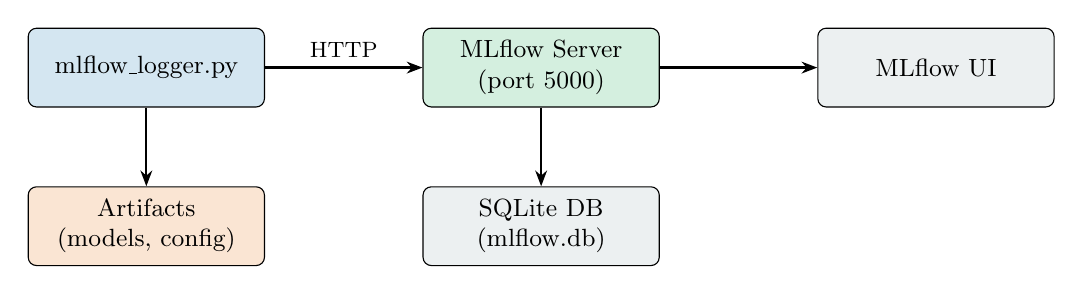
\begin{tikzpicture}[
    node distance=1cm,
    box/.style={draw, rounded corners=3pt, minimum width=3cm, minimum height=1cm, align=center, font=\small},
    arrow/.style={-{Stealth[length=2mm]}, thick}
]

\node[box, fill=primaryblue!20] (logger) {mlflow\_logger.py};
\node[box, fill=secondarygreen!20, right=2cm of logger] (server) {MLflow Server\\(port 5000)};
\node[box, fill=lightgray, below=1cm of server] (db) {SQLite DB\\(mlflow.db)};
\node[box, fill=lightgray, right=2cm of server] (ui) {MLflow UI};
\node[box, fill=accentorange!20, below=1cm of logger] (artifacts) {Artifacts\\(models, config)};

\draw[arrow] (logger) -- node[above, font=\footnotesize] {HTTP} (server);
\draw[arrow] (server) -- (db);
\draw[arrow] (server) -- (ui);
\draw[arrow] (logger) -- (artifacts);

\end{tikzpicture}
\caption{MLflow integration architecture}
\end{figure}

\subsection{Logged Information}

\begin{lstlisting}[style=pythonstyle]
with mlflow.start_run() as run:
    # 1. Log metrics
    mlflow.log_metrics({
        "accuracy": accuracy,
        "precision": precision,
        "recall": recall,
    })

    # 2. Log fairness metrics (per gender)
    mlflow.log_metric(f"accuracy_{gender}", group_acc)
    mlflow.log_metric(f"selection_rate_{gender}", rate)

    # 3. Log parameters
    mlflow.log_params({
        "n_estimators": 200,
        "max_depth": 4,
        "with_gender": True,
        "data_source": "data/credit_dataset1.csv",
    })

    # 4. Log model with signature
    signature = infer_signature(X_test, y_pred)
    mlflow.sklearn.log_model(pipeline, "model",
                             signature=signature)

    # 5. Log artifacts
    mlflow.log_artifact("model/xgb_credit_model.pkl")
    mlflow.log_artifact("config.py")
\end{lstlisting}

% ============================================================================
% SECTION 9: DEPLOYMENT
% ============================================================================
\section{Deployment Infrastructure}

\subsection{Deployment Options}

The platform supports two deployment modes:

\begin{table}[H]
\centering
\begin{tabular}{@{}lll@{}}
\toprule
\textbf{Mode} & \textbf{Use Case} & \textbf{Configuration} \\
\midrule
Docker Compose & Local development, testing & \texttt{docker-compose.yml} \\
Kubernetes & Production, scaling & \texttt{k8s/k8s-manifests.yaml} \\
\bottomrule
\end{tabular}
\end{table}

\subsection{Docker Compose Architecture}

\begin{figure}[H]
\centering
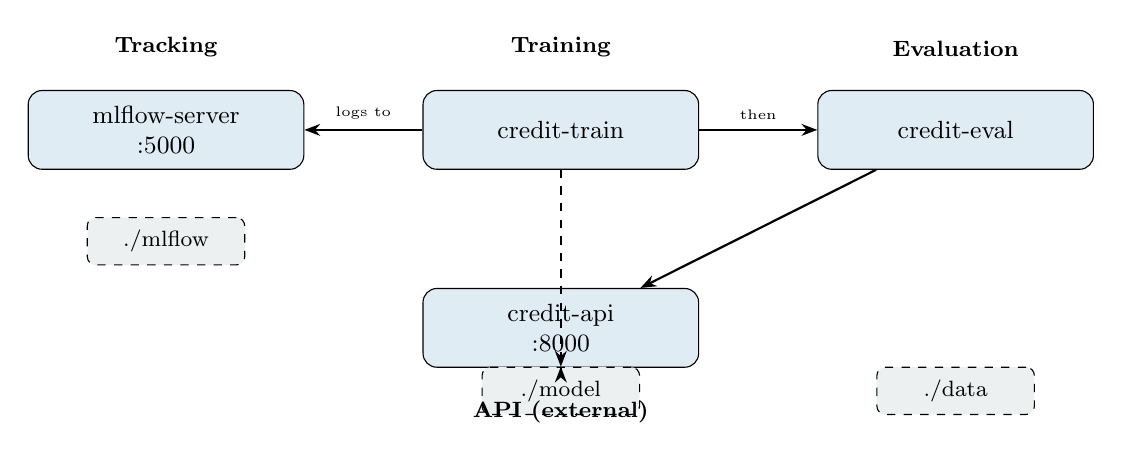
\begin{tikzpicture}[
    node distance=0.8cm,
    container/.style={draw, rounded corners=5pt, minimum width=3.5cm, minimum height=1cm, align=center, font=\small, fill=primaryblue!15},
    volume/.style={draw, rounded corners=3pt, minimum width=2cm, minimum height=0.6cm, align=center, font=\footnotesize, fill=lightgray, dashed},
    arrow/.style={-{Stealth[length=2mm]}, thick}
]

% Containers
\node[container] (mlflow) {mlflow-server\\:5000};
\node[container, right=1.5cm of mlflow] (train) {credit-train};
\node[container, right=1.5cm of train] (eval) {credit-eval};
\node[container, below=1.5cm of train] (api) {credit-api\\:8000};

% Volumes
\node[volume, below=0.6cm of mlflow] (mlflowvol) {./mlflow};
\node[volume, below=2.5cm of train] (modelvol) {./model};
\node[volume, below=2.5cm of eval] (datavol) {./data};

% Arrows (dependencies)
\draw[arrow] (train) -- node[above, font=\tiny] {logs to} (mlflow);
\draw[arrow] (train) -- node[above, font=\tiny] {then} (eval);
\draw[arrow] (eval) -- (api);
\draw[arrow, dashed] (train) -- (modelvol);
\draw[arrow, dashed] (api) -- (modelvol);

% Labels
\node[above=0.3cm of mlflow, font=\footnotesize\bfseries] {Tracking};
\node[above=0.3cm of train, font=\footnotesize\bfseries] {Training};
\node[above=0.3cm of eval, font=\footnotesize\bfseries] {Evaluation};
\node[below=0.3cm of api, font=\footnotesize\bfseries] {API (external)};

\end{tikzpicture}
\caption{Docker Compose service architecture}
\end{figure}

\textbf{Usage:}
\begin{lstlisting}[language=bash, style=yamlstyle]
# Build and run all services
docker-compose up --build

# Access services:
# - MLflow UI: http://localhost:5000
# - API: http://localhost:8000/predict
\end{lstlisting}

\subsection{Kubernetes Architecture}

The Kubernetes deployment provides production-grade features:

\begin{figure}[H]
\centering
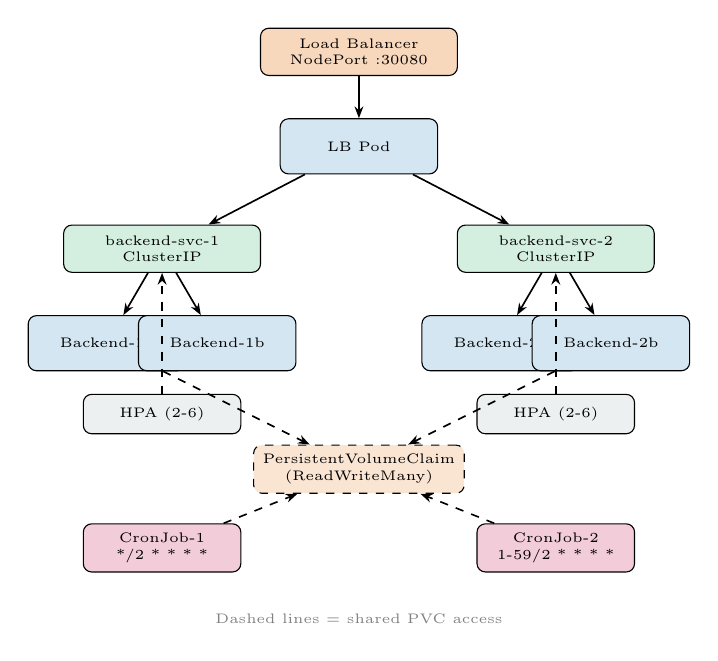
\begin{tikzpicture}[
    node distance=0.6cm,
    pod/.style={draw, rounded corners=3pt, minimum width=2cm, minimum height=0.7cm, align=center, font=\tiny, fill=primaryblue!20},
    svc/.style={draw, rounded corners=3pt, minimum width=2.5cm, minimum height=0.6cm, align=center, font=\tiny, fill=secondarygreen!20},
    pvc/.style={draw, rounded corners=3pt, minimum width=2cm, minimum height=0.6cm, align=center, font=\tiny, fill=accentorange!20, dashed},
    hpa/.style={draw, rounded corners=3pt, minimum width=2cm, minimum height=0.5cm, align=center, font=\tiny, fill=lightgray},
    cron/.style={draw, rounded corners=3pt, minimum width=2cm, minimum height=0.6cm, align=center, font=\tiny, fill=purple!20},
    arrow/.style={-{Stealth[length=1.5mm]}, semithick}
]

% External
\node[svc, fill=accentorange!30] (lb) at (0,4) {Load Balancer\\NodePort :30080};

% Load balancer pod
\node[pod] (lbpod) at (0,2.8) {LB Pod};

% Services
\node[svc] (svc1) at (-2.5,1.5) {backend-svc-1\\ClusterIP};
\node[svc] (svc2) at (2.5,1.5) {backend-svc-2\\ClusterIP};

% Backend pods (replicas)
\node[pod] (b1a) at (-3.2,0.3) {Backend-1a};
\node[pod] (b1b) at (-1.8,0.3) {Backend-1b};
\node[pod] (b2a) at (1.8,0.3) {Backend-2a};
\node[pod] (b2b) at (3.2,0.3) {Backend-2b};

% HPA
\node[hpa] (hpa1) at (-2.5,-0.6) {HPA (2-6)};
\node[hpa] (hpa2) at (2.5,-0.6) {HPA (2-6)};

% PVC
\node[pvc] (pvc) at (0,-1.3) {PersistentVolumeClaim\\(ReadWriteMany)};

% CronJobs
\node[cron] (cron1) at (-2.5,-2.3) {CronJob-1\\*/2 * * * *};
\node[cron] (cron2) at (2.5,-2.3) {CronJob-2\\1-59/2 * * * *};

% Arrows
\draw[arrow] (lb) -- (lbpod);
\draw[arrow] (lbpod) -- (svc1);
\draw[arrow] (lbpod) -- (svc2);
\draw[arrow] (svc1) -- (b1a);
\draw[arrow] (svc1) -- (b1b);
\draw[arrow] (svc2) -- (b2a);
\draw[arrow] (svc2) -- (b2b);
\draw[arrow, dashed] (hpa1) -- (svc1);
\draw[arrow, dashed] (hpa2) -- (svc2);
\draw[arrow, dashed] (b1a) -- (pvc);
\draw[arrow, dashed] (b2b) -- (pvc);
\draw[arrow, dashed] (cron1) -- (pvc);
\draw[arrow, dashed] (cron2) -- (pvc);

% Legend
\node[font=\tiny, text=gray] at (0,-3.2) {Dashed lines = shared PVC access};

\end{tikzpicture}
\caption{Kubernetes deployment architecture}
\label{fig:k8s-arch}
\end{figure}

\textbf{Key Kubernetes Components:}

\begin{table}[H]
\centering
\small
\begin{tabular}{@{}llp{6cm}@{}}
\toprule
\textbf{Resource} & \textbf{Count} & \textbf{Purpose} \\
\midrule
PersistentVolumeClaim & 1 & Shared storage for model files (ReadWriteMany) \\
CronJob & 2 & Periodic model retraining (every 2 min, offset) \\
Deployment & 3 & 2 backend deployments + 1 load balancer \\
Service (ClusterIP) & 2 & Internal routing to backend pods \\
Service (NodePort) & 1 & External access on port 30080 \\
HorizontalPodAutoscaler & 2 & Auto-scale backends (2-6 replicas, 60\% CPU) \\
\bottomrule
\end{tabular}
\end{table}

\subsection{Model Hot-Reload}

The \texttt{backend.py} implements zero-downtime model updates:

\begin{lstlisting}[style=pythonstyle]
# Periodic model reload (every 30 seconds)
def _periodic_reload(interval: int):
    while True:
        time.sleep(interval)
        load_model()  # Reload from shared PVC

# Background thread for hot-reload
_reload_thread = threading.Thread(
    target=_periodic_reload,
    args=(RELOAD_SECS,),
    daemon=True
)
_reload_thread.start()
\end{lstlisting}

\subsection{Deploying to Kubernetes}

\begin{lstlisting}[language=bash, style=yamlstyle]
# Apply all manifests
kubectl apply -f k8s/k8s-manifests.yaml

# Verify deployments
kubectl get pods -l app=credit-backend
kubectl get svc

# Test the API
curl http://<NODE-IP>:30080/predict \
  -H "Content-Type: application/json" \
  -d '{"Age": 35, "Sex": "male", ...}'
\end{lstlisting}

% ============================================================================
% SECTION 10: API DOCUMENTATION
% ============================================================================
\section{API Documentation}

\subsection{Endpoints}

\begin{table}[H]
\centering
\begin{tabular}{@{}llp{6cm}@{}}
\toprule
\textbf{Endpoint} & \textbf{Method} & \textbf{Description} \\
\midrule
\texttt{/predict} & POST & Submit credit application for risk prediction \\
\texttt{/model-info} & GET & Get current model metadata \\
\texttt{/health} & GET & Health check for load balancer/K8s probes \\
\bottomrule
\end{tabular}
\end{table}

\subsection{POST /predict}

\textbf{Request Body:}
\begin{lstlisting}[style=pythonstyle]
{
    "Age": 35,
    "Sex": "male",
    "Job": 2,
    "Housing": "own",
    "Saving_accounts": "moderate",
    "Checking_account": 15.0,
    "Credit_amount": 5000.0,
    "Duration": 24,
    "Purpose": "car"
}
\end{lstlisting}

\textbf{Response:}
\begin{lstlisting}[style=pythonstyle]
{
    "Risk": "Good",
    "Probability": 0.73,
    "dataset_id": "1",
    "model_trained_at": "2024-01-15 10:30:00",
    "host": "backend-pod-abc123"
}
\end{lstlisting}

\subsection{GET /model-info}

\textbf{Response:}
\begin{lstlisting}[style=pythonstyle]
{
    "status": "active",
    "dataset_id": "1",
    "last_trained_at": "2024-01-15 10:30:00",
    "metrics": {"accuracy": 0.82, "precision": 0.79},
    "feature_names": ["Age", "Sex", ...],
    "model_type": "Pipeline",
    "host": "backend-pod-abc123"
}
\end{lstlisting}

% ============================================================================
% SECTION 11: MODIFICATION GUIDE
% ============================================================================
\section{Modification Guide}

This section provides guidance on common modifications you may want to make.

\subsection{Changing the Dataset}

\begin{enumerate}
    \item Place your new CSV file in \texttt{data/}
    \item Edit \texttt{config.py}:
\begin{lstlisting}[style=pythonstyle]
DATA_PATH = "data/your_new_dataset.csv"
MODEL_PATH = os.path.join(MODEL_DIR, "your_model.pkl")
\end{lstlisting}
    \item Update feature columns if schema differs:
\begin{lstlisting}[style=pythonstyle]
CATEGORICAL_COLS = ["feature1", "feature2", ...]
NUMERICAL_COLS = ["feature3", "feature4", ...]
TARGET = "your_target_column"
\end{lstlisting}
\end{enumerate}

\subsection{Changing the Model}

To use a different classifier:

\begin{lstlisting}[style=pythonstyle]
# In train.py, replace XGBClassifier:
from sklearn.ensemble import RandomForestClassifier

model = RandomForestClassifier(
    n_estimators=100,
    max_depth=10,
    random_state=config.RANDOM_STATE,
)
\end{lstlisting}

\textbf{Note}: For SHAP compatibility, tree-based models (XGBoost, RandomForest, LightGBM) work best with \texttt{TreeExplainer}.

\subsection{Changing Protected Attribute}

To analyze fairness on a different attribute:

\begin{lstlisting}[style=pythonstyle]
# In config.py:
PROTECTED_ATTR = "Age_Group"  # or any categorical column

# You may need to create age groups first:
df["Age_Group"] = pd.cut(df["Age"],
    bins=[0, 30, 50, 100],
    labels=["Young", "Middle", "Senior"]
)
\end{lstlisting}

\subsection{Disabling Gender in Model}

To train a model without gender as a feature:

\begin{lstlisting}[style=pythonstyle]
# In config.py:
WITH_GENDER = False

# This automatically:
# - Removes "Sex" from CATEGORICAL_COLS
# - Skips fairness evaluation
# - Updates the training pipeline
\end{lstlisting}

\subsection{Adding New Fairness Metrics}

To add custom fairness metrics:

\begin{lstlisting}[style=pythonstyle]
# In evaluate.py, extend the MetricFrame:
from fairlearn.metrics import true_positive_rate

mf = MetricFrame(
    metrics={
        "selection_rate": selection_rate,
        "false_positive_rate": false_positive_rate,
        "true_positive_rate": true_positive_rate,  # Added
        # Add custom metrics here
    },
    y_true=y_test,
    y_pred=y_pred,
    sensitive_features=s_test,
)
\end{lstlisting}

\subsection{Modifying XGBoost Hyperparameters}

\begin{lstlisting}[style=pythonstyle]
# In train.py:
model = XGBClassifier(
    n_estimators=500,       # More trees
    max_depth=6,            # Deeper trees
    learning_rate=0.05,     # Slower learning
    subsample=0.8,          # More dropout
    colsample_bytree=0.8,   # Feature sampling
    min_child_weight=3,     # Regularization
    gamma=0.1,              # Min split loss
    reg_alpha=0.1,          # L1 regularization
    reg_lambda=1.0,         # L2 regularization
)
\end{lstlisting}

\subsection{Adding New API Endpoints}

\begin{lstlisting}[style=pythonstyle]
# In backend.py or inference.py:
@app.get("/feature-importance")
def feature_importance():
    if current_model is None:
        raise HTTPException(status_code=503)

    # Get XGBoost feature importance
    booster = current_model.named_steps["model"].get_booster()
    importance = booster.get_score(importance_type="gain")
    return {"feature_importance": importance}
\end{lstlisting}

\subsection{Kubernetes Scaling Configuration}

\begin{lstlisting}[style=yamlstyle]
# In k8s/k8s-manifests.yaml, modify HPA:
spec:
  minReplicas: 3        # Increase minimum
  maxReplicas: 10       # Increase maximum
  metrics:
  - type: Resource
    resource:
      name: cpu
      target:
        type: Utilization
        averageUtilization: 50  # Scale earlier
\end{lstlisting}

% ============================================================================
% SECTION 12: FILE REFERENCE
% ============================================================================
\section{Complete File Reference}

\begin{longtable}{@{}p{4cm}p{9cm}@{}}
\toprule
\textbf{File} & \textbf{Description} \\
\midrule
\endfirsthead
\toprule
\textbf{File} & \textbf{Description} \\
\midrule
\endhead
\bottomrule
\endfoot

\multicolumn{2}{l}{\textbf{Core Python Files}} \\
\midrule
\texttt{config.py} & Central configuration: paths, feature definitions, data loading \\
\texttt{train.py} & Model training with sklearn Pipeline and XGBoost \\
\texttt{evaluate.py} & Performance metrics, SHAP, LIME, fairness analysis \\
\texttt{mlflow\_logger.py} & MLflow experiment logging with fairness audit \\
\texttt{inference.py} & Simple FastAPI inference server \\
\texttt{backend.py} & Production backend with model hot-reload \\
\texttt{load\_balancer.py} & Flask round-robin load balancer \\
\texttt{model\_trainer.py} & K8s CronJob-compatible training script \\

\midrule
\multicolumn{2}{l}{\textbf{Docker Configuration}} \\
\midrule
\texttt{docker-compose.yml} & Local multi-service orchestration \\
\texttt{docker/Dockerfile.train} & Training container image \\
\texttt{docker/Dockerfile.evaluate} & Evaluation container image \\
\texttt{docker/Dockerfile.inference} & API inference container \\
\texttt{docker/Dockerfile.backend} & K8s backend container \\
\texttt{docker/Dockerfile.mlflow} & MLflow server container \\
\texttt{docker/Dockerfile.loadbalancer} & Load balancer container \\
\texttt{docker/Dockerfile.trainer} & K8s trainer container \\

\midrule
\multicolumn{2}{l}{\textbf{Kubernetes Configuration}} \\
\midrule
\texttt{k8s/k8s-manifests.yaml} & Complete K8s deployment manifests \\

\midrule
\multicolumn{2}{l}{\textbf{Requirements}} \\
\midrule
\texttt{requirements.txt} & Main project dependencies \\
\texttt{docker/requirements/*.txt} & Container-specific dependencies \\

\midrule
\multicolumn{2}{l}{\textbf{Data}} \\
\midrule
\texttt{data/credit\_dataset1.csv} & Primary credit risk dataset \\
\texttt{data/credit\_dataset2.csv} & Secondary credit risk dataset \\

\midrule
\multicolumn{2}{l}{\textbf{Outputs}} \\
\midrule
\texttt{model/*.pkl} & Trained model artifacts \\
\texttt{visualizations/*.png} & Generated plots and charts \\
\texttt{mlflow/mlflow.db} & MLflow tracking database \\

\end{longtable}

% ============================================================================
% SECTION 13: SUMMARY
% ============================================================================
\section{Summary}

XAI-Lab demonstrates a complete, production-ready ML platform that addresses the key challenges of deploying ML in regulated domains:

\begin{enumerate}
    \item \textbf{Explainability}: SHAP and LIME provide both global and local explanations
    \item \textbf{Fairness}: Comprehensive fairness auditing using Fairlearn
    \item \textbf{Reproducibility}: MLflow tracks experiments, parameters, and artifacts
    \item \textbf{Scalability}: Kubernetes deployment with auto-scaling
    \item \textbf{Reliability}: Model hot-reload, health checks, and graceful shutdown
\end{enumerate}

The modular architecture allows easy customization of:
\begin{itemize}
    \item Datasets and feature engineering
    \item Machine learning models
    \item Fairness metrics and protected attributes
    \item Deployment configurations
\end{itemize}

This platform serves as both a learning resource and a foundation for production ML systems requiring transparency and accountability.

% ============================================================================
% APPENDIX
% ============================================================================
\appendix

\section{Quick Start Commands}

\subsection{Local Development (Docker Compose)}
\begin{lstlisting}[language=bash, style=yamlstyle]
# Clone and navigate to project
cd XAI-Lab

# Build and start all services
docker-compose up --build

# Access:
# - MLflow UI: http://localhost:5000
# - API: http://localhost:8000

# Test prediction
curl -X POST http://localhost:8000/predict \
  -H "Content-Type: application/json" \
  -d '{
    "Age": 35,
    "Sex": "male",
    "Job": 2,
    "Housing": "own",
    "Saving_accounts": "moderate",
    "Checking_account": 15,
    "Credit_amount": 5000,
    "Duration": 24,
    "Purpose": "car"
  }'
\end{lstlisting}

\subsection{Kubernetes Deployment}
\begin{lstlisting}[language=bash, style=yamlstyle]
# Start Minikube (if local)
minikube start

# Apply manifests
kubectl apply -f k8s/k8s-manifests.yaml

# Wait for pods
kubectl get pods -w

# Get service URL
minikube service credit-load-balancer-service --url

# Test prediction
curl -X POST <URL>/predict \
  -H "Content-Type: application/json" \
  -d '{"Age": 35, ...}'
\end{lstlisting}

\section{Troubleshooting}

\begin{table}[H]
\centering
\small
\begin{tabular}{@{}p{4cm}p{8cm}@{}}
\toprule
\textbf{Issue} & \textbf{Solution} \\
\midrule
Model not found & Wait for training to complete; check \texttt{./model/} directory \\
SHAP slow & Use \texttt{TreeExplainer} for tree models; reduce test set size \\
Fairness skipped & Check \texttt{WITH\_GENDER = True} in config.py \\
K8s pods pending & Check PVC provisioner; verify storage class exists \\
API 503 error & Model still loading; check readiness probe logs \\
\bottomrule
\end{tabular}
\end{table}

\end{document}
